\chapter{Preliminaries}
\label{ch:Foundations}

\section{Confidential Computing}
\label{sec:Foundations:ConfComputing}
Confidential Computing means the protection of data during computation by performing those computations in attested Trusted Execution Environments (TEE). Similarly to Trusted Computing, Confidential Computing is predominantly a marketing term and has no single definition. The following tries to establish the definition as it will be used in this thesis. Unlike Trusted Computing, which aims to establish integrity of hardware and software, Confidential Computing also aims to guarantee the authenticity. Using TEEs in the lowest layer of hardware reduces the number of trusted parties. In this case, a party could be a hardware or software vendor. Security in one abstraction layer of the compute stack is only as strong as the layers below it if no other measures are used to prevent access. Homomorphic encryption gives some additional security guarantees even if the underlying layers are not trusted. Figure \ref{fig:computestack} shows a basic compute stack. A bug in the hypervisor, if present, can affect the execution of the operating system and, in the worst case read or change the data in use.
\begin{figure}
\centering
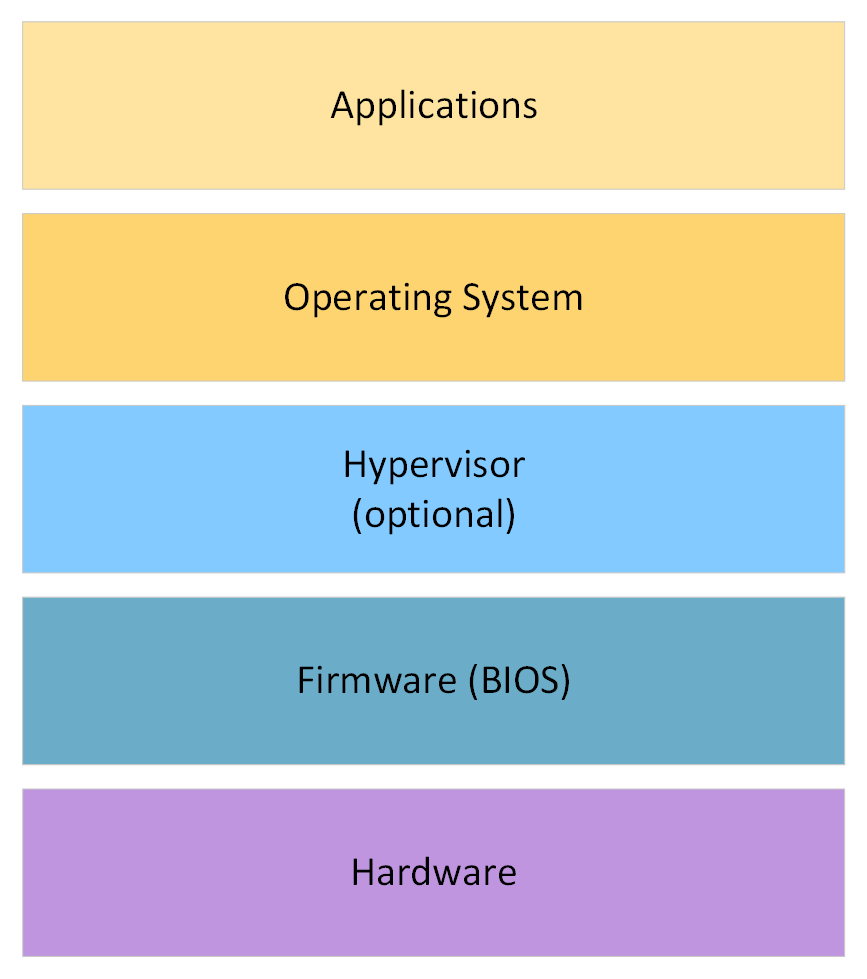
\includegraphics[width=0.5\textwidth]{figures/ComputeStack.png}
\caption{A rudimentary Compute Stack. Most layers can be split up further if needed to}
\label{fig:computestack}
\end{figure}Security in higher layers can be bypassed from lower layers. Security solutions at the hardware level can remove the operating system, device drivers, and more from the list of trusted parties. Confidential Computing protects data in use by performing computation in a hardware-based Trusted Execution Environment (TEE). A TEE is, as defined by the Confidential Computing Consortium, an environment that provides assurance in three different properties:
\begin{itemize} 
    \item \guillemotright Data confidentiality: Unauthorized entities cannot view data while it is in use within the TEE
    \item Data integrity: Unauthorized entities cannot alter the data while it is in use within the TEE.
    \item Code integrity: Unauthorized entities cannot alter the code executing in the TEE.\guillemotleft \cite{noauthor_ccc_outreach_whitepaper_updated_november_2022pdf_2023}
\end{itemize} 
In the context of Confidential Computing, unauthorized entities include, but are not limited to, other applications on the host, the host operating system itself, as well as the hypervisor, the infrastructure owner, and anyone else with physical hardware access. 
Combined, these three attributes provide an assurance that the data are kept confidential and the calculations that are performed are correct.
Depending on the specific TEE used, there might be additional security properties, but the TEEs covered in this thesis do not have more\cite{noauthor_ccc_outreach_whitepaper_updated_november_2022pdf_2023}.
\section{Trusted Domain Extension}
One implementation of TEEs by Intel is called Trusted Domain Extensions (TDX). This section gives an overview of its building blocks, its system architecture, memory protection mechanisms, I/O model, attestation, and future features.
\subsection{TDX Building Blocks}
\label{sec:tdxBuildingBlocks}
TDX combines and extends several existing Intel technologies, including Virtualization Technology (VT), Total Memory Encryption (TME), and Software Guard Extensions (SGX). This section will provide a brief overview of the technologies and how they are used. The general information is from \cite{cheng_intel_2023}.
\subsubsection{Software Guard Extension}
Intel introduced SGX in 2015 with its sixth generation core processors. It was intended to protect against memory bus snooping and cold boot attacks. It is still in use today to protect code and data within a so called enclave, which is a secure container \todo{enclave erklären} \cite{intel_corporation_overview--intel-sgx-enclave_nodate}. SGX aims to protect the integrity and confidentiality of the computation inside an enclave. The RAM of an enclave can only be accessed by authorized code. SGX uses hardware-based memory encryption to protect the enclave. Any unauthorized attempt to access the memory will result in an exception. SGX offers both local and, more importantly, remote attestation to verify the integrity of enclaves. Local attestation establishes trust between two local enclaves, and remote attestation verifies trustworthiness to a third party entity. More on attestation can be found in \ref{TDX attestation} On the same platform, TDX and SGX are within the same Trusted Computing Base (TCB).  Therefore, they can attest each other locally\cite{intel_corporation_intel_2024-1}, which will become important for TDX in \ref{Pre-Attestation setup}. During its lifetime Intel SGX has had many security issues, with most of them being preventable by the application developer themself. \url{https://sgx.fail/}\cite{sgxfail} provides an overview of known issues at the time of writing and ways to mitigate them. The same source also contains an overview of attacks that can only be prevented with microcode updates by Intel itself. \todo{Wovor kann und will SGX nicht schützen?}
\subsubsection{Intel Virtualization Technology}
Intel Virtualization Technology (Intel VT) is a set of hardware-assisted virtualization features in Intel processors that can provide improved performance, isolation, and security compared to software-based virtualization. Intel VTs features include virtualization of the CPU, memory, I/O.
Intel processors contain, depending on the architecture, either VT-x or VT-i instructions. The latter being only used on the discontinued Itanium architecture. Processors with VT-x have a special instruction set called Virtual Machine Extensions (VMX), which enables virtualization control. Virtualization allows the usage of multiple isolated Virtual Machines on the same hardware. It can also allow multiple different Operating Systems to be running in these VMs\cite{intel_corporation_intel_nodate}. VMX has two different execution modes: VMX root mode, used by the hypervisor, and VMX nonroot mode, used by the guest VMs. VMX utilises a Second Level Address Translation called Extended Page Table (EPT), which aims to remove the overhead from software-managed page tables \cite{uhlig_intel_2005}. The TDX Module (TDXM) runs in the new Secure Arbitration Mode (SEAM) VMX root and the TDs run in the nonroot mode. The biggest change from normal VMX to SEAM VMX is the usage of an additional Extended Page Table. With VMX the hypervisor holds only one table per guest kernel, the TDXM has two per guest TD. A protected one for private memory and another unprotected one for shared memory.
With TDX being a virtual machine-based TEE, it depends on VT to ensure isolation between its Trusted Domains (TDs)\cite{cheng_intel_2023}.
\subsubsection{Intel Total Memory Encryption}
Intel Total Memory Encryption (TME) is a security measure designed to protect against attackers who have physical access to the memory of a computer or direct access via a host system and attempt to steal data. TME encrypts the entire computer's memory using a single key, which is generated at boot-time by a hardened hardware-based random number generator. Memory encryption is performed by encryption engines on each memory controller, using the, for storage encryption, recommended standard AES-XTS of the US National Institute of Standards and Technologies \cite{morris_dworkin_recommendation_2015} and the German Federal Office for Information Security with 128 or 256-bit keys\cite[~p. 24]{bundesamt_fur_sicherheit_in_der_informationstechnik_cryptographic_2023}. The encryption engines sit directly in between the memory controllers and the CPU cache, meaning the data inside the SoC remains plain text, while the data inside the memory is always encrypted. Total Memory Encryption Multi Key (TME-MK, also sometimes MKTME) extends TME to support multiple keys and memory encryption at page granularity. To use TME-MK in virtualized environments, the hypervisor must be trusted, which violates the threat model for confidential computing, which will be explained in more detail in chapter \ref{Security Analysis}. Therefore, in TDX, the TDX Module is responsible for controlling the memory encryption of TDs. Figure \ref{fig:component-overview} shows what a TD encapsulates. The TDX Module requests the processor to generate a new key when building a new TD and binds the two together via its Key Management Tables. The TDX module then utilizes MKTME to encrypt the cache lines. The TDXM stores cryptographic keys only in its Key Encryption Tables, thus never exposing them to the outside\cite{cheng_intel_2023}. \todo{TME Schuttziele + MKTME Schutzziele, wie werden diese erreicht?}

\subsection{TDX System Architecture}
Fig \ref{fig:component-overview} illustrates the runtime architecture of TDX. It is made up of two key components: 
\begin{itemize}
    \item TDX-enabled processors, which offer architectural functionalities like hard-ware-assisted virtualization, memory encryption/integrity protection, and the ability to certify TEE platforms,
    \item TDX Module, an Intel-signed and CPU-attested software module that leverages the features of TDX-enabled processors to facilitate the construction, execution, and termination of TDs while enforcing the security guarantees. 
\end{itemize} The TDX Module provides two sets of interface functions, host-side interface functions for a TDX-enlightened hypervisor and guest-side interface functions for TDs. It is loaded and executed in the SEAM RANGE, which is a portion of system memory reserved via UEFI/BIOS. The P-SEAM Loader, which also resides in the SEAM RANGE, can install and update the TDX Module. More information on the loading process can be found in \cite{noauthor_white_nodate} and \cite{noauthor_tdx-module-10-public-specpdf_nodate}.
A TDX-enlightened hypervisor operates in the traditional VMX root mode and utilizes the SEAMCALL instruction to call host-side interface functions (function names start with TDH) of the TDX Module. Upon execution of the SEAMCALL instruction, the logical processor transitions from the VMX root mode to the SEAM VMX root mode and starts executing code within the TDX Module. Once the TDX module has completed its task, it returns to the hypervisor in VMX root mode by executing the SEAMRET instruction. On the other hand, TDs run in the SEAM VMX nonroot mode. TDs can trap into the TDX Module either through a TD exit by invoking the TDCALL instruction or triggered by some external event, e.g. an external interrupt or exception. In both cases, the logical processor transitions from the SEAM VMX nonroot mode into the SEAM VMX root mode and starts executing in the context of the TDX Module.
\begin{figure}
\centering
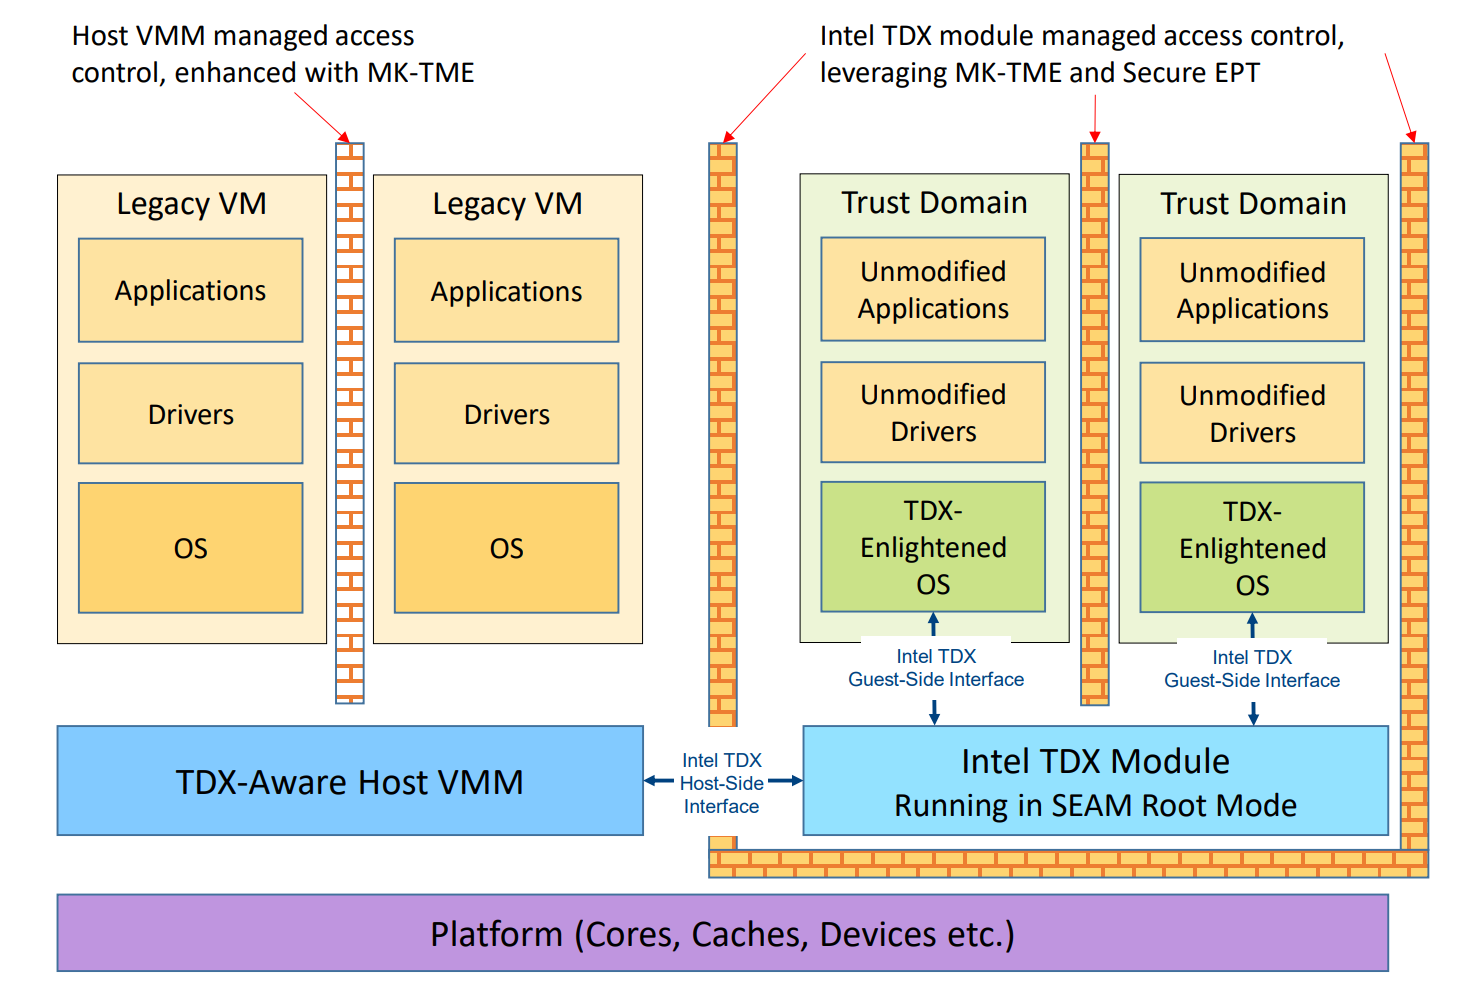
\includegraphics[width=\textwidth]{figures/TDX-Component-Overview}
\caption{TDX Component Overview taken from \cite[p.~19]{noauthor_tdx-module-10-public-specpdf_nodate}. Shown here is an extension of the Compute Stack in Fig. \ref{fig:computestack} with the colors corresponding to the non-TDX variants.}
\label{fig:component-overview}
\end{figure}
\subsection{TDX Key Generation and TD encryption}
The Host Hypervisor or Virtual Machine Manager (host VMM), which explicitly is not part of the TDX module but is aware of it calls the TDH.SYS.KEY.CONFIG function during startup, which configures the TDX modules global private key on the current CPU package \cite{intel_corporation_intel-tdx-module-15-abi-spec-348551001pdf_2024}. \todo{Was genau heißt configures private key on current package?} The host VMM can create a new guest TD by allocating and initializing a TD root control structure. The host assigns the TD a Host Key ID (HKID), which can be used to tag the memory accesses made by the TD\cite{noauthor_tdx-module-10-public-specpdf_nodate}. Subsequently, the host VMM calls the MKTME hardware, which encrypts the specified memory using a hardware-generated encryption key\cite{noauthor_multi-key-total-memory-encryption-spec-14pdf_nodate}. The VMM of the TD host configures the MKTME hardware by calling the TDH.MNG.KEY.CONFIG function on each CPU package. This will program the encryption key into the MKTME encryption engines\cite{noauthor_tdx-module-10-public-specpdf_nodate}. At this point, the TD private memory section is created and accessible by the TD. The VMM can then use Intel TDXM interface functions to create control structures. 
\subsection{TDX Attestation}
\label{TDX attestation}
Hardware attestation is a process that ensures the integrity and trustworthiness of hardware components in a computing system. It involves verifying the identity and expected behavior of hardware components connected to the motherboard. This verification is done by checking identification codes and comparing them to expected values. Attestation is necessary to establish trust for a challenger, that the used hardware is as expected. Without attestation the security assurances by TDX are not guaranteed. 
\label{Pre-Attestation setup}
Before any attestation request can be answered the platform itself needs to register. This is done by creating a shared platform key using the hardware-keys of the different CPUs on the platform. This shared platform key is then encrypted using those hardware-keys and flashed into the BIOS. After booting the host platform accesses this certificate, called platform manifest, and registers the plattform at the Intel SGX Registration service. During this registration Intel checks the validity of the platform manifest. From this platform manifest the public key of the Provisioning Certification Enclave (PCE) is then signed by Intel and returned.

Complementary to the three provisions required by the Confidential Computing Consortium, in the context of attestation according to \cite{sardar_demystifying_2021}, the four most interesting properties are:

\label{FourProperties}
\textit{Integrity}: Claims within Evidence represent the present condition of the Attester and contain components such as identity fields. Therefore, it is crucial to prevent the adversary from altering Claims while they are being transported from the Attester to the Verifier. Typically, the integrity of Claims is safeguarded through digital signatures utilizing an Attestation Key. If the correspondence assertion holds true, it signifies that the adversary cannot modify the variables of agreement without being detected. 

\textit{Freshness}: The freshness of Evidence is crucial because otherwise an attacker has the ability to replay authentic Evidence from a previous session while simultaneously altering the state of the Attester.

\textit{Secrecy}: It must be ensured that the adversary does not have access to attestation-related keys or secrets shared between Attester and Verifier

\textit{Authentication}: The Verifier must ensure it communicates with the intended Attester. Informally, if the Verifier receives the public key of the Target Environment, this uniquely matches the public key generated within the Target Environment.

Hardware attestation establishes trust into the hardware but not the software being executed. The Attestation does however generate a quote that contains additional information on the TD and the software being executed. Trusting the Quote does not mean trust with the TD is established but only that the information in the quote is to be trusted. This establishes the environment of the TD, mainly the specific hardware and the TDX Module. With the additional information about the VM and the Image in the Quote verification might be possible but the implementation of that is left to the software developer. More information on this can be found in \ref{Identity}.
The TD attestation protocol involves six key entities: the Quoting Enclave (QE), the host Virtual Machine Manager (VMM), the guest trust domain (TD), the Intel TDX module, the CPU hardware and the challenger. The QE is an Intel-provided enclave that signs the report body after its successful verification to create a remotely verifiable Quote. The VMM is an untrusted hypervisor that manages Virtual Machines. The guest TD is an enhanced Virtual Machine that is initialized and measured at boot time. The TDX module is Intel-provided software that is signed by Intel and manages the interaction between the TD and the VMM. It is also part of the attestation metadata. The CPU hardware generates and verifies the report. Lastly, the challenger (also known as the relying party) is the remote party that performs the attestation verification.
\begin{figure}
\centering
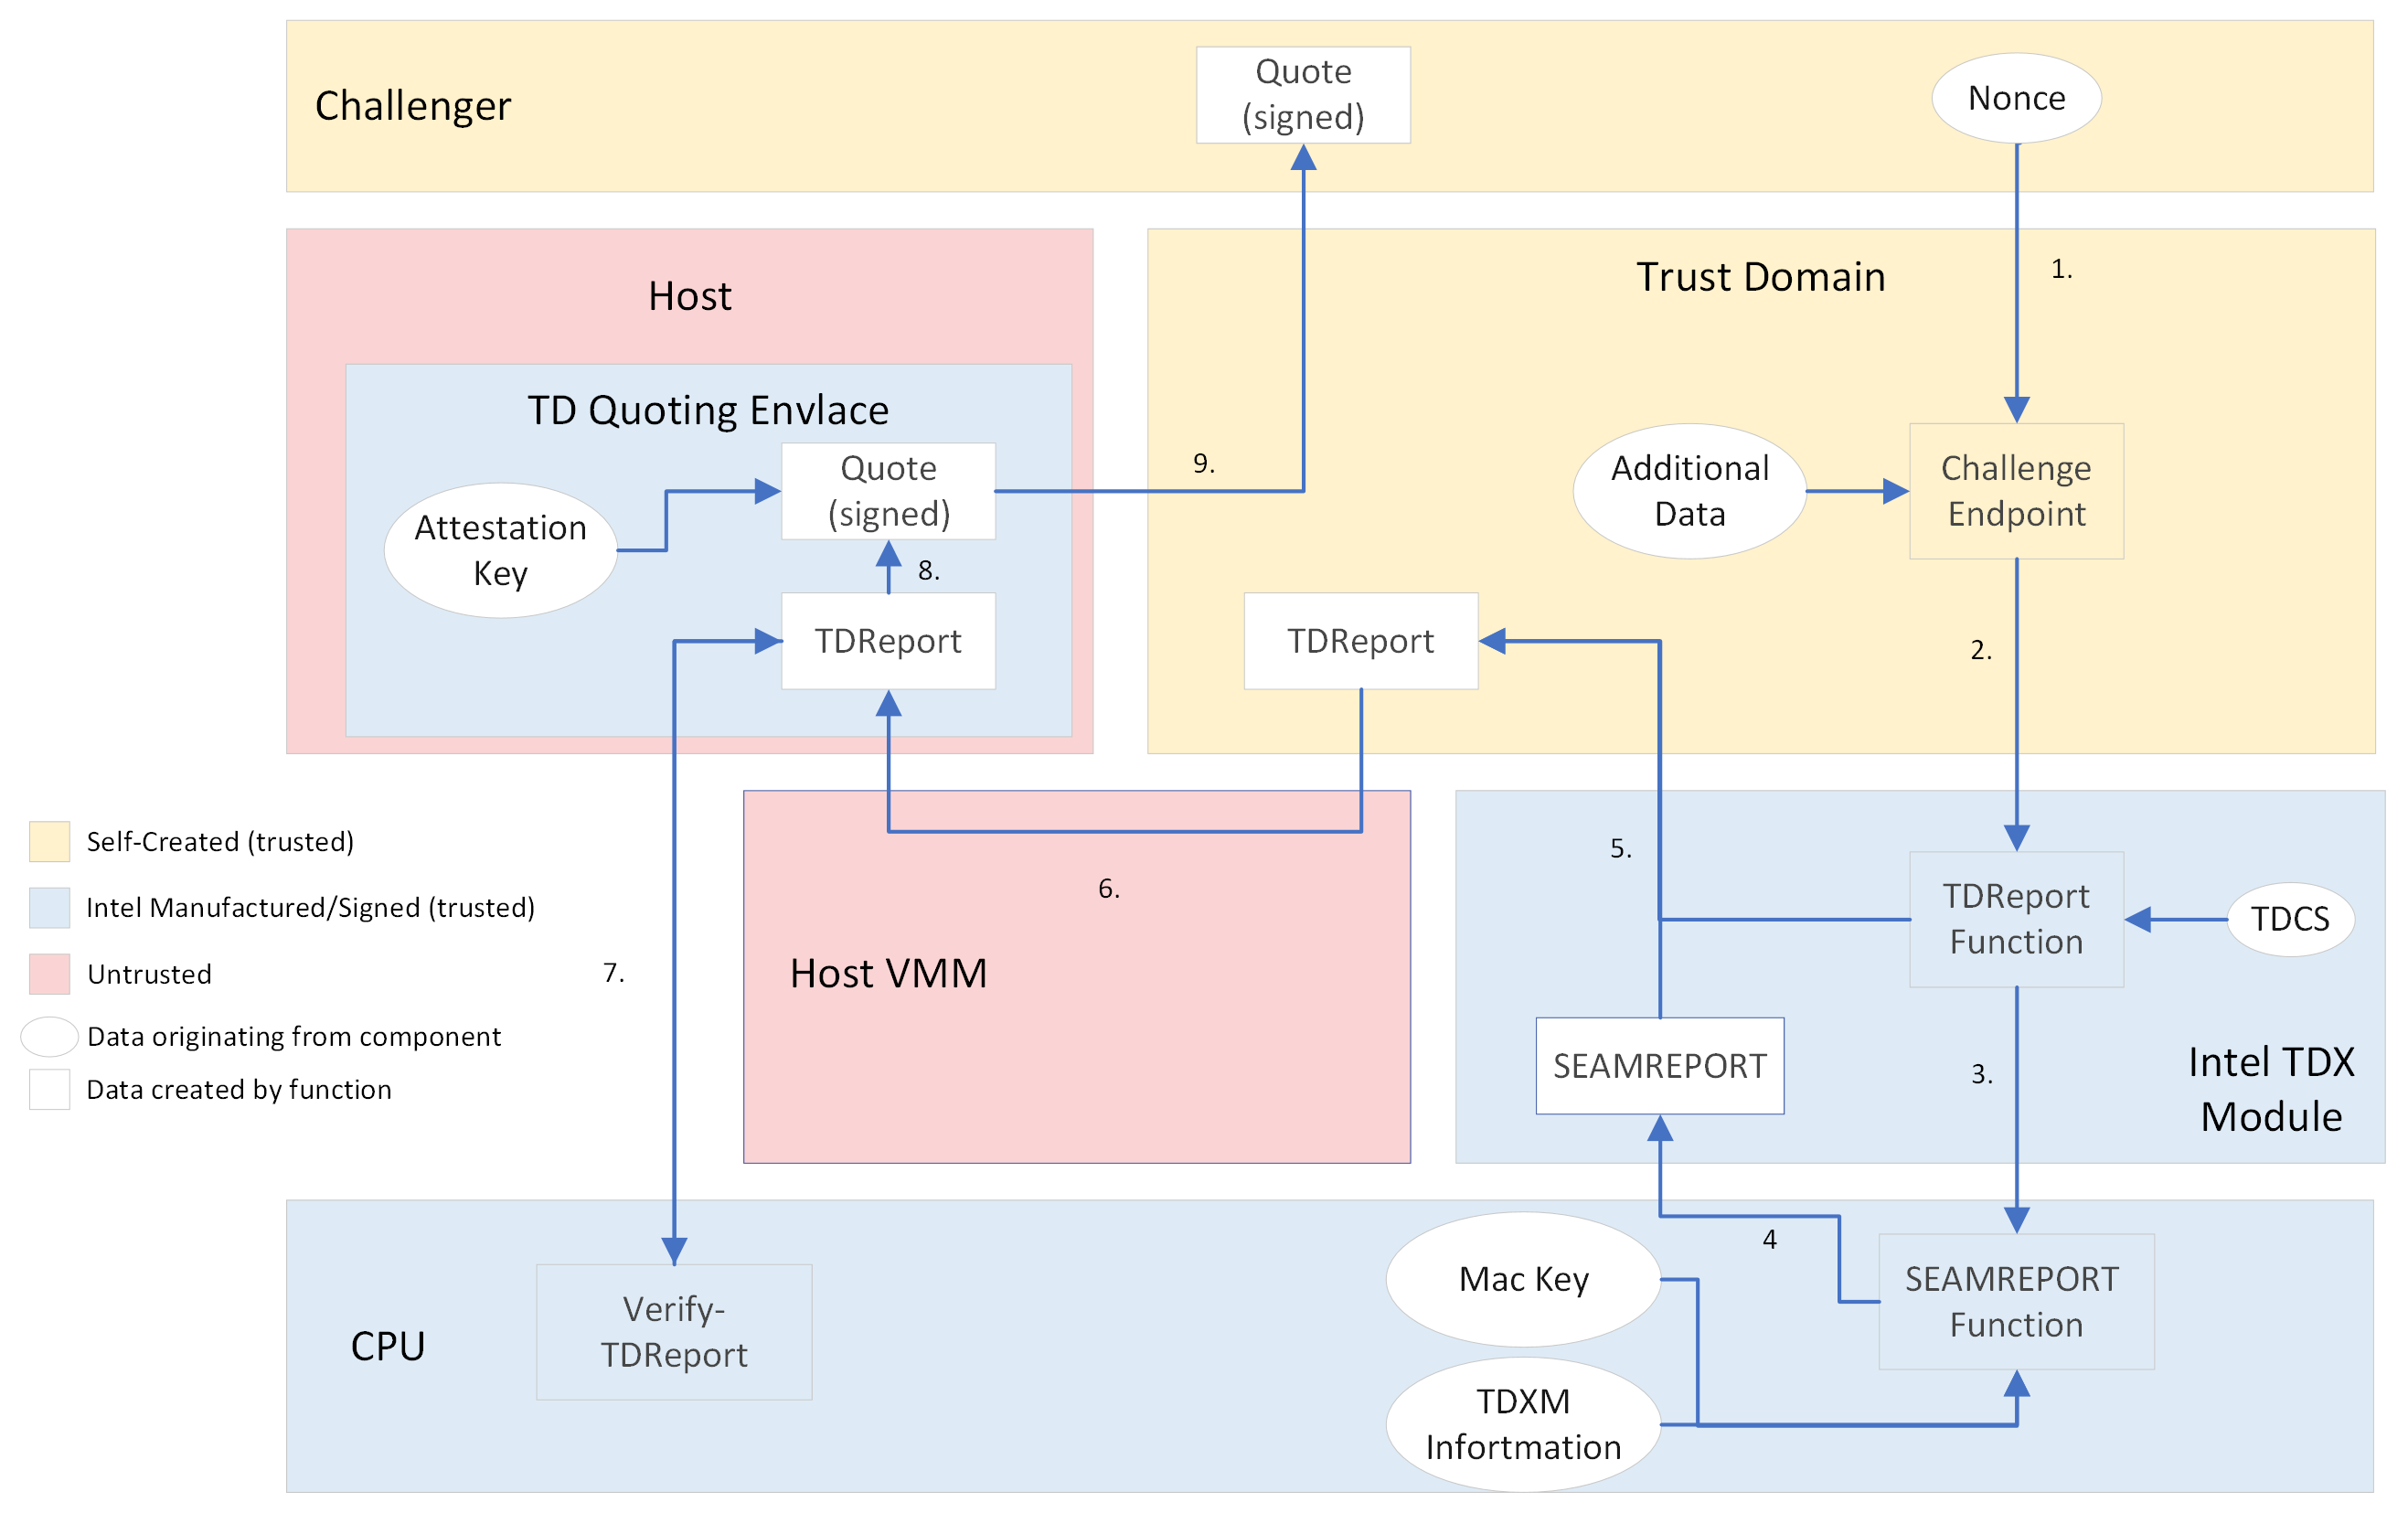
\includegraphics[width=\textwidth]{figures/Attestation-einfach.png}
\caption{A simplified SGX-based TD attestation flow. Adapted from \cite[p.~111]{noauthor_tdx-module-10-public-specpdf_nodate}}
\label{fig:EasyAttestation}
\end{figure}
Figure \ref{fig:EasyAttestation} shows a rudimentary TDX attestation flow with trusted and untrusted entities as well as their boundaries. The challenger requests a quote from the guest TD for challenge. He can include a one-time key, called nonce to prevent replay attacks. A quote is all the information necessary to attest to a specific set of hardware. After receiving the request the guest TD can supply additional runtime data, which is important to verify the authenticity of the TD, and will then send a request via a character device to the TDX module. This report contains data the TDX module holds about the TD, most importantly measurements relating to the creation of the TD, and the data that was supplied by the TD. To prevent issues with the data transfer via the untrusted Host VMM the CPU has a Message Authentication Key (MAC) from the TD QE, which it uses to encrypt the TDReport. The TD QE now calls the CPU again to verify the integrity of the TDReport.
To create a chain of trust, which can only be accessed via Intel, the Attestation key was previously signed by the PCE key, which was signed by Intel. This means that the Quote can in the end only be decrypted via an Intel service.

\begin{figure}
\centering
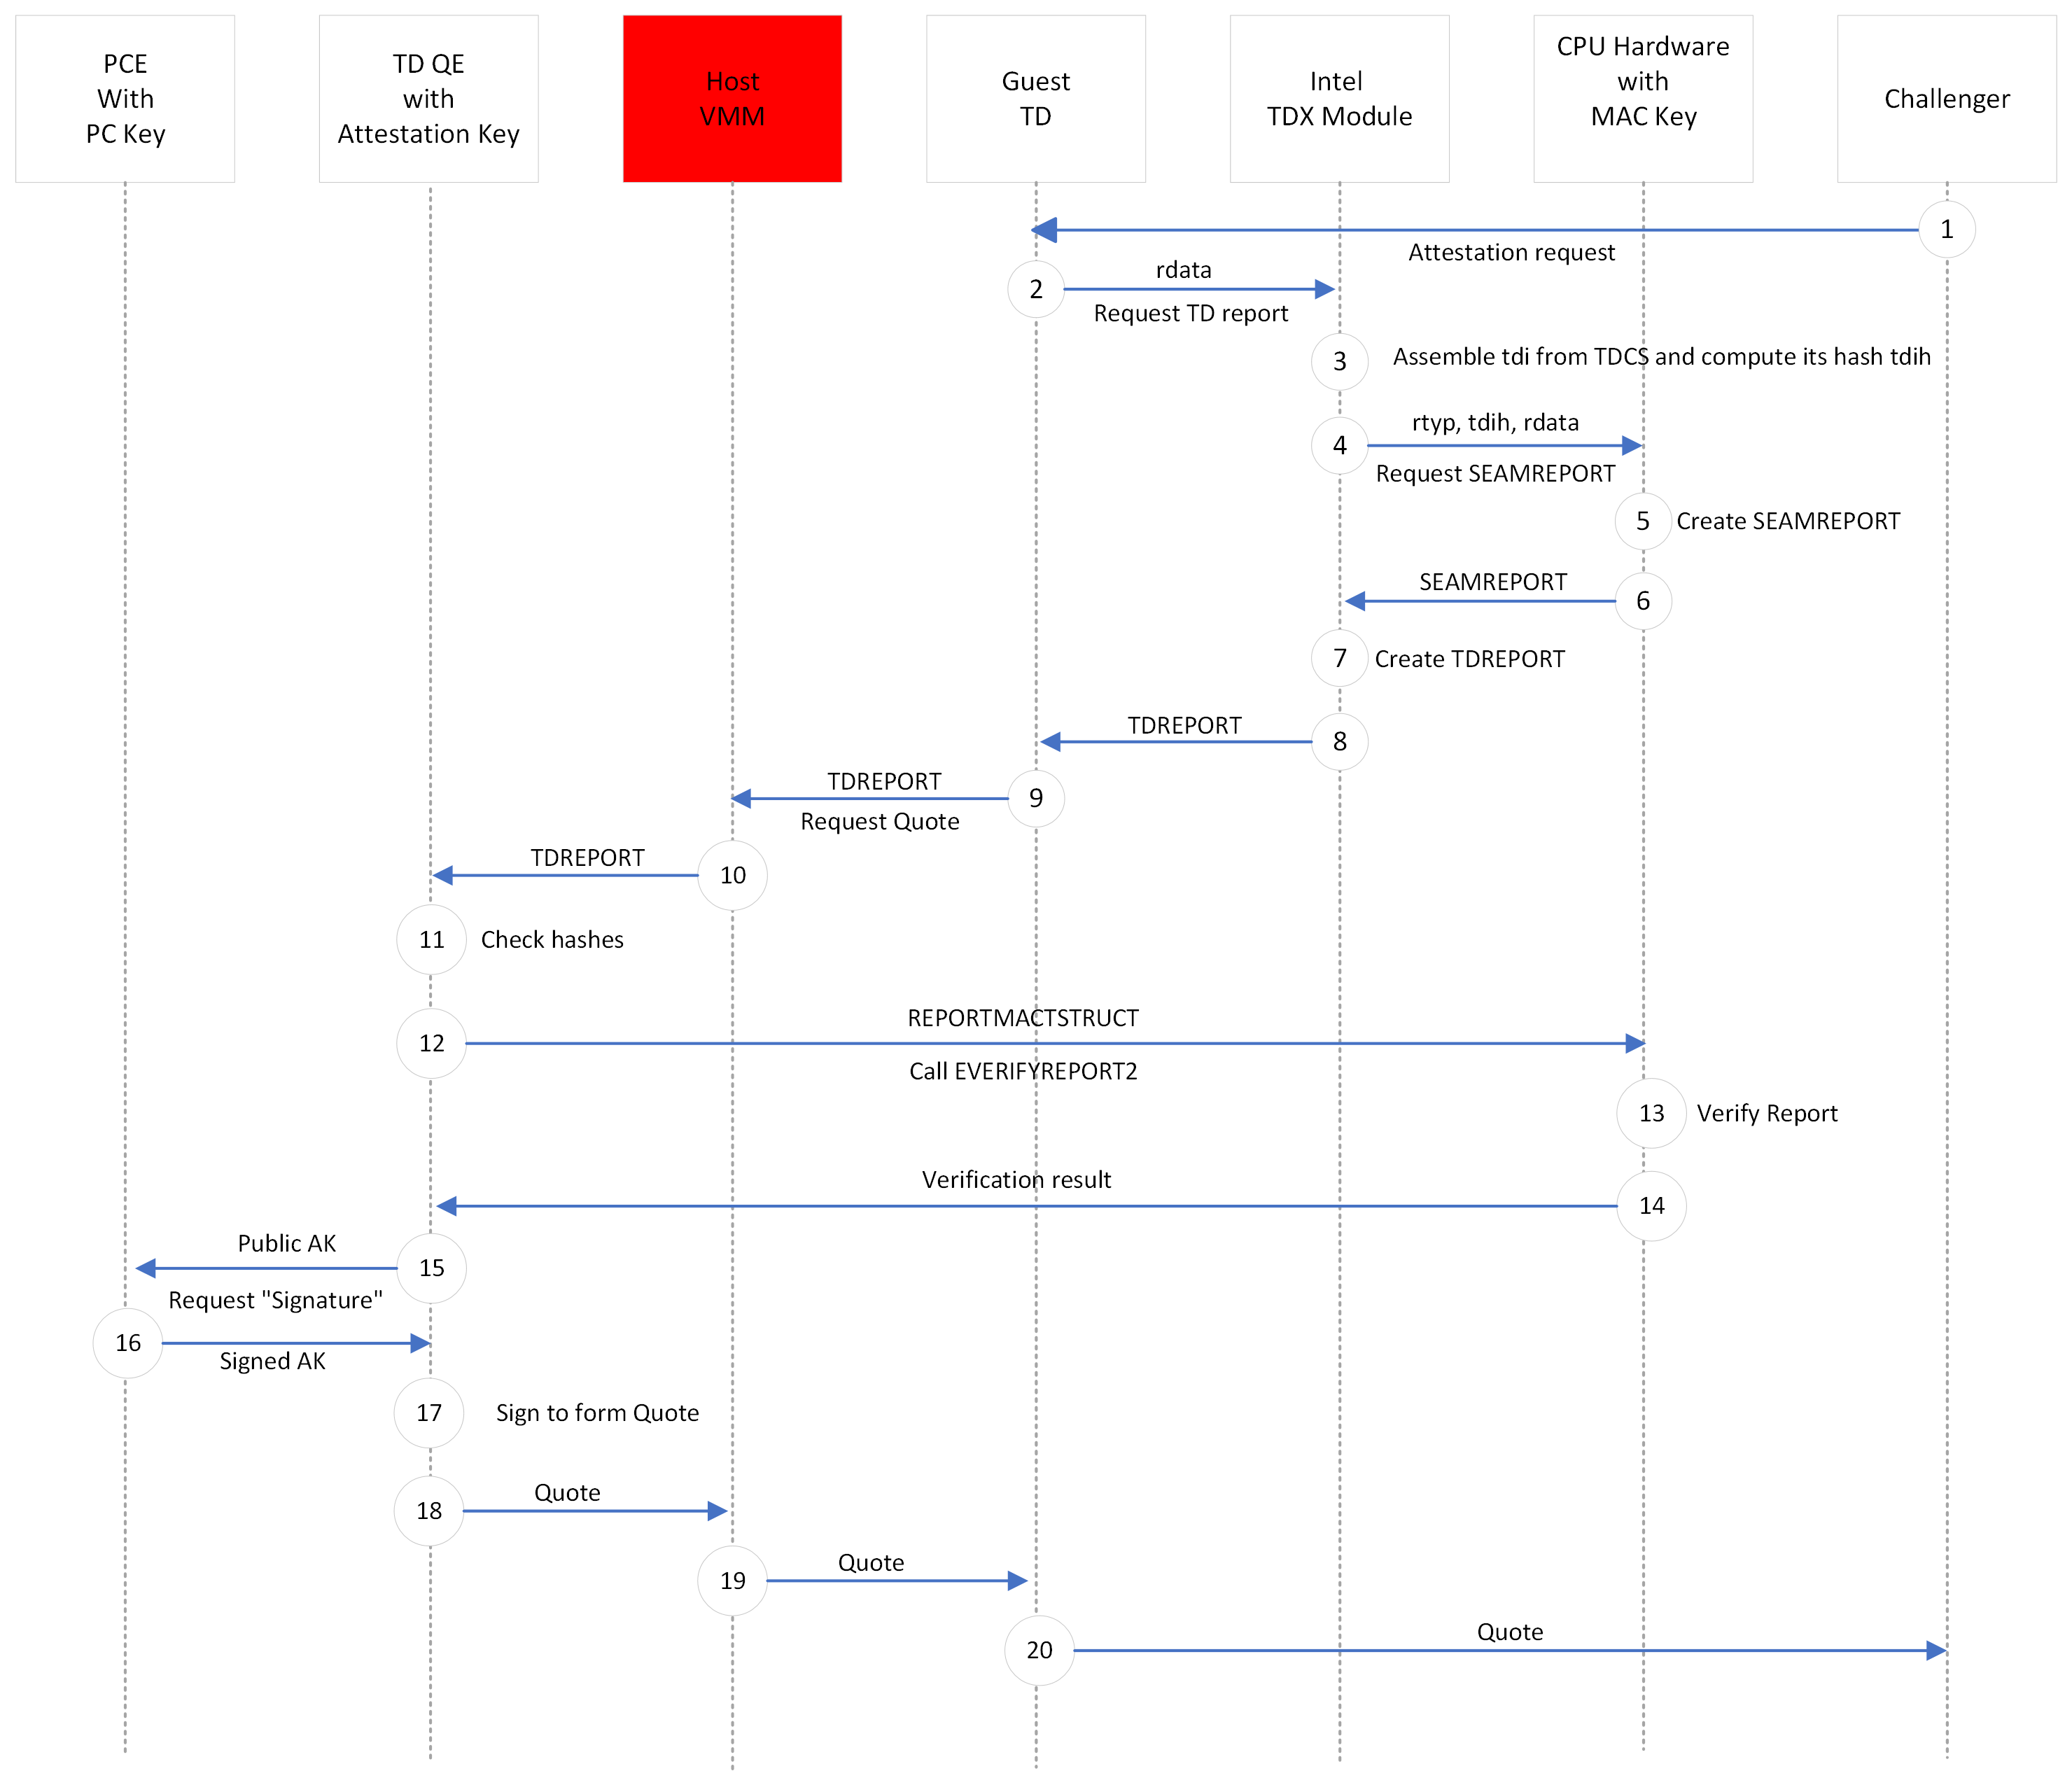
\includegraphics[width=\textwidth]{figures/Attestation Diagram (1).png}
\caption{Intel TDX Attestation flow diagram. Text above the arrow represents data being sent, text below function calls. The Host VMM in red is untrusted. Adapted from \cite{sardar_demystifying_2021}}
\label{fig:QuoteGeneration}
\end{figure}
The following will now explain each step in more technical detail, while using Figure \ref{fig:QuoteGeneration} as reference. 
TDX includes a set of major functions explained here. \textit{Sign} represents the Elliptic Curve Digital Signature Algorithm signature over the message with the specified signature key. 
Calculating the \textit{hash} means computing the SHA384 of the input. \textit{Hmac} is HMAC\_SHA256 of the message with the specified key. The message is not extractable if hmac is considered a pseudorandom function, which in practice appears to be true\cite{bellare_new_2006}.
\newcommand\setItemnumber[1]{\setcounter{enumi}{\numexpr#1-1\relax}}
\begin{enumerate}
\item The challenger initiates the attestation process by sending a challenge request to the Guest TD. This can include a nonce to prevent replay attacks\cite{sardar_formal_2023}.
\item TD calls TDG.MR.REPORT by sending the hash of its public key and the challenge to the TDXM (using rdata). This is generally done via the character device tdx\_guest in Linux
\item TDXM assembles TD information data structure tdi from Trust Domain Control Structure (TCDS) and computes its SHA384 hash tdih. The TCDS contains the following information:
\begin{itemize}
    \item Fields designed to control the TD operation as a whole (e.g., a counter of the number of VCPUs currently running). 
    \item Fields designed to control the execution control of the TD (debugability, CPU features available to the TD, etc.). 
    \item Registers filled with static and runtime measurements. 
    \item EPTP: as designed, a pointer (HPA) to the TD’s secure Extended Page Table (EPT) root page and EPT attributes
    \item Model Specific Register (MSR) bitmaps, designed to be used by all the TD’s VCPUs. 
    \item A page filled with zeros, designed to be used in cases where the Intel TDX Module needs a read-only constant 0 page encrypted with the TD’s private key.
\end{itemize}
\item TDXM calls SEAMOPS[SEAMREPORT] with tdih and rdata
\item[5. \& 6.] CPU generates SEAMREPORT smr  with rms (red) and tcbi (purple) \ref{fig:tdr} and returns it to the TDX module. This importantly contains measurements about the TDX module and about the TDX module signer, in this case Intel.
\setItemnumber{7}
\item TDXM builds tdr with smr, res4, and tdi. Content for the entire tdr can be seen in Figure \ref{fig:tdr}
\begin{figure}
\centering
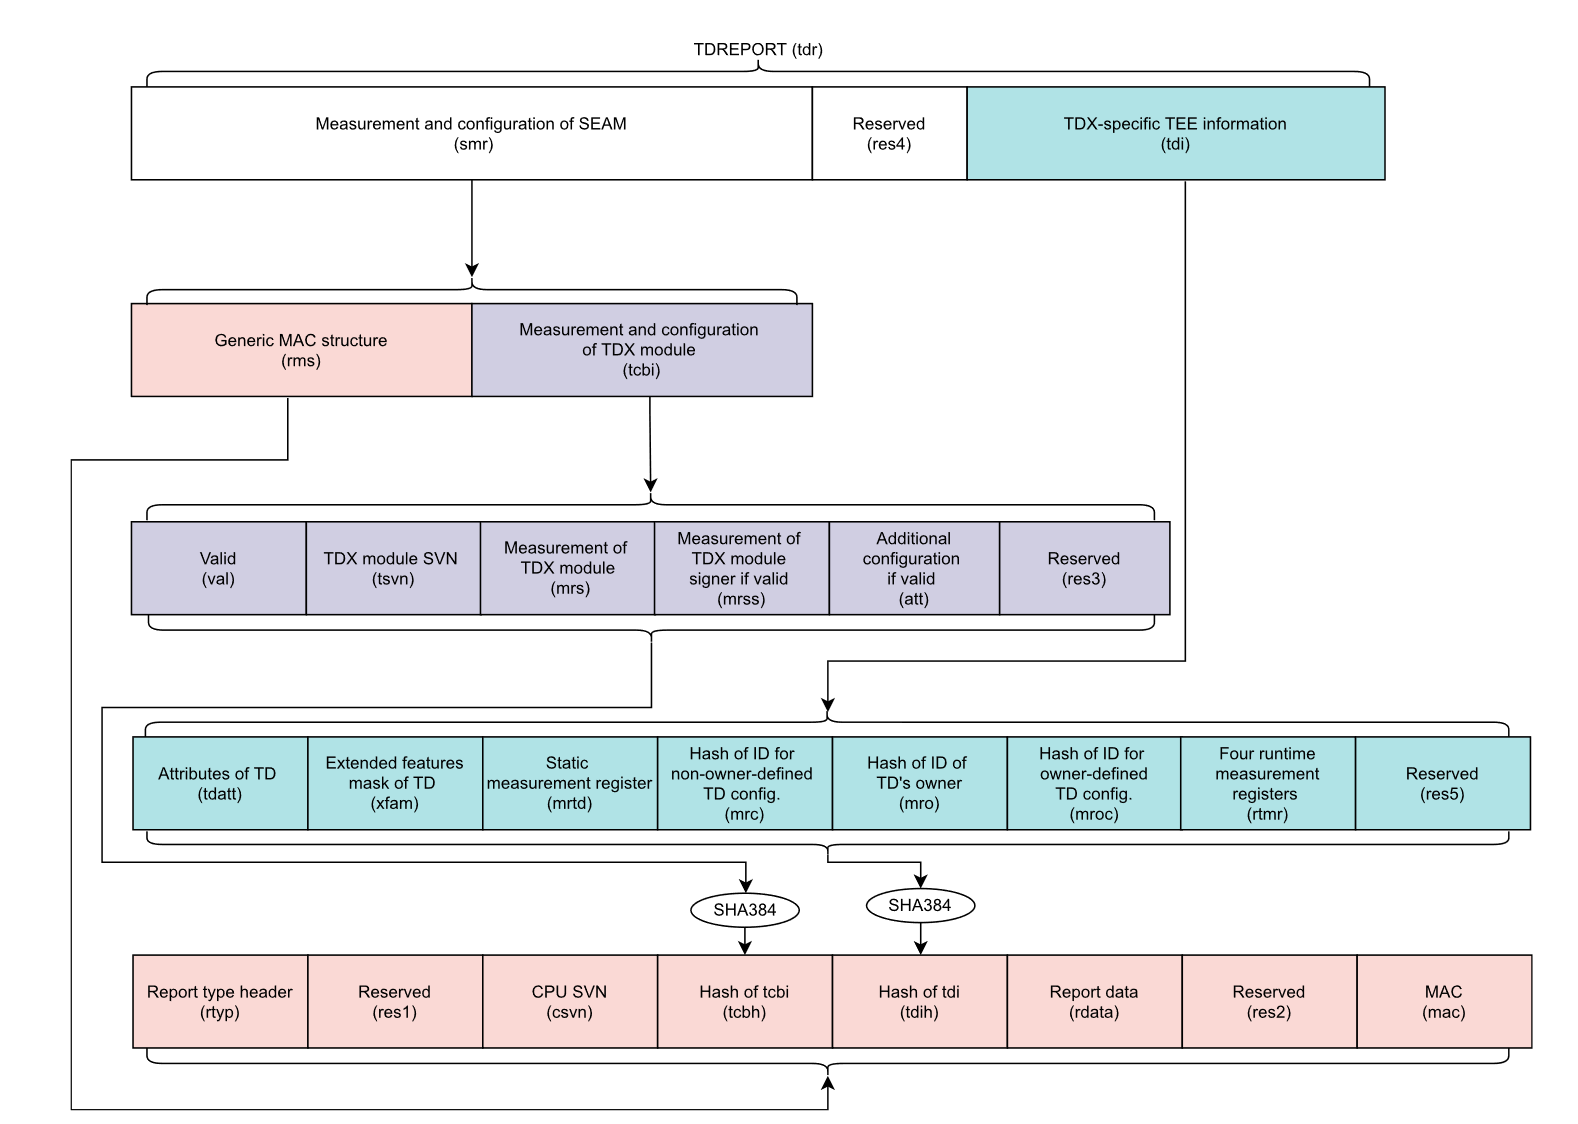
\includegraphics[width=\textwidth]{figures/tdr.png}
\caption{An overview of the component of the TDREPORT taken from \cite{sardar_demystifying_2021}}
\label{fig:tdr}
\end{figure}
\item TDXM sends tdr to the Guest TD
\item[9 \& 10.]The Guest TD sends tdr to the TD Quoting enclave, via the untrusted VMM
\setItemnumber{11}
\item TD QE verifies the hashes in report
\item Rms (part of smr, red in Fig \ref{fig:tdr}) is used as an argument in the ENCLU[EVERIFYREPORT2] cpu function. 
\item[13. \& 14.] CPU performs the verification of rms and returns the result to the TD QE. The verification consists of three main steps: 
\begin{enumerate}
\item verify that the header rtyp in the report is correct, 
\item verify that the CPUSVN csvn is a valid value, and 
\item compute the MAC over the fields in the report body rptbody using the MAC key MACkey, and verify that the computed MAC matches the value in the field mac of the received report (represented as receivedMAC)
\end{enumerate}
\setItemnumber{15}
\item The PCE and the TD QE do local attestation to verify that they are running on the same platform (this is not shown in detail) and then the Provisioning Certification Enclave signs the public key of the Attestation Key with its Provisioning Certification Key which in turn is signed by Intel during the platform registration. 
\ref{Pre-Attestation setup}
\item TD QE replaces the MAC with a Quote defined as <rptbody, (sign(AK, rptbody))>.
\item[18. \& 19.] Quote is sent to TD, VMM is untrusted → Sent by public channel
\setItemnumber{18}
\item TD sends quote to relying party(RP)
\end{enumerate}
The challenger can now verify the Signature on the Quotebody by going back the chain of trust rooted at Intel. This verification is based on the Data Center Attestation Primitives (DCAP) which will be explored later on in \ref{Security Analysis}. After verification the challenger can now send a secret encrypted with the public key of the TD to the TD establishing a common secret for further secure communication. If the TD did not include a public key in its quote section \ref{Establishing_a_secure_connection} contains further information on how to establish a secure connection. According to \cite{sardar_formal_2023} using ProVerif, this ensures integrity for the tcbi, tdi and rdata. It also ensures freshness and secrecy. Authentication does not hold as long as secure communication via TLS or similar is not established.

\section{Related Work}
TDX has been looked at a fair amount of times already. In particular, a nearly complete security analysis of its hardware and the low-level TDX software by Aktas et al. at Google \cite{aktas_intel_nodate}. They limited their analysis to just the host-side without looking at TD user or developer issues down the line. Similarly, Sardar et al. formally verified TDX attestation in \cite{sardar_demystifying_2021}. They looked at the theoretical security of a perfect implementation. Knauth et al. introduced a way to create a secure channel using Intel SGX \cite{knauth_integrating_2019}, this will be used as the basis to establishing a secure channel to the TD in this thesis. Cheng et al. briefly mention this as well, but their focus was more generally on the TDX architecture \cite{cheng_intel_2023}. This thesis explores the feasibility of those for an average user, as well as its security assumptions and pitfalls. Lefeuvre et al. have looked at difficulties and issues with safe and confidential I/O \cite{lefeuvre_towards_2023}, this will only be briefly touched upon in this thesis. Delignat-Lavaud et al. looked at issues pertaining the TCB of confidential services. Their information was used in this thesis to look at the feasibility of using CC for the average user. Their consensus was picked up in this thesis that while CC is great in theory, the practice is lacking.

